% Options for packages loaded elsewhere
% Options for packages loaded elsewhere
\PassOptionsToPackage{unicode}{hyperref}
\PassOptionsToPackage{hyphens}{url}
\PassOptionsToPackage{dvipsnames,svgnames,x11names}{xcolor}
%
\documentclass[
  letterpaper,
]{article}
\usepackage{xcolor}
\usepackage[margin=1in]{geometry}
\usepackage{amsmath,amssymb}
\setcounter{secnumdepth}{5}
\usepackage{iftex}
\ifPDFTeX
  \usepackage[T1]{fontenc}
  \usepackage[utf8]{inputenc}
  \usepackage{textcomp} % provide euro and other symbols
\else % if luatex or xetex
  \usepackage{unicode-math} % this also loads fontspec
  \defaultfontfeatures{Scale=MatchLowercase}
  \defaultfontfeatures[\rmfamily]{Ligatures=TeX,Scale=1}
\fi
\usepackage{lmodern}
\ifPDFTeX\else
  % xetex/luatex font selection
\fi
% Use upquote if available, for straight quotes in verbatim environments
\IfFileExists{upquote.sty}{\usepackage{upquote}}{}
\IfFileExists{microtype.sty}{% use microtype if available
  \usepackage[]{microtype}
  \UseMicrotypeSet[protrusion]{basicmath} % disable protrusion for tt fonts
}{}
\makeatletter
\@ifundefined{KOMAClassName}{% if non-KOMA class
  \IfFileExists{parskip.sty}{%
    \usepackage{parskip}
  }{% else
    \setlength{\parindent}{0pt}
    \setlength{\parskip}{6pt plus 2pt minus 1pt}}
}{% if KOMA class
  \KOMAoptions{parskip=half}}
\makeatother
% Make \paragraph and \subparagraph free-standing
\makeatletter
\ifx\paragraph\undefined\else
  \let\oldparagraph\paragraph
  \renewcommand{\paragraph}{
    \@ifstar
      \xxxParagraphStar
      \xxxParagraphNoStar
  }
  \newcommand{\xxxParagraphStar}[1]{\oldparagraph*{#1}\mbox{}}
  \newcommand{\xxxParagraphNoStar}[1]{\oldparagraph{#1}\mbox{}}
\fi
\ifx\subparagraph\undefined\else
  \let\oldsubparagraph\subparagraph
  \renewcommand{\subparagraph}{
    \@ifstar
      \xxxSubParagraphStar
      \xxxSubParagraphNoStar
  }
  \newcommand{\xxxSubParagraphStar}[1]{\oldsubparagraph*{#1}\mbox{}}
  \newcommand{\xxxSubParagraphNoStar}[1]{\oldsubparagraph{#1}\mbox{}}
\fi
\makeatother


\usepackage{longtable,booktabs,array}
\newcounter{none} % for unnumbered tables
\usepackage{calc} % for calculating minipage widths
% Correct order of tables after \paragraph or \subparagraph
\usepackage{etoolbox}
\makeatletter
\patchcmd\longtable{\par}{\if@noskipsec\mbox{}\fi\par}{}{}
\makeatother
% Allow footnotes in longtable head/foot
\IfFileExists{footnotehyper.sty}{\usepackage{footnotehyper}}{\usepackage{footnote}}
\makesavenoteenv{longtable}
\usepackage{graphicx}
\makeatletter
\newsavebox\pandoc@box
\newcommand*\pandocbounded[1]{% scales image to fit in text height/width
  \sbox\pandoc@box{#1}%
  \Gscale@div\@tempa{\textheight}{\dimexpr\ht\pandoc@box+\dp\pandoc@box\relax}%
  \Gscale@div\@tempb{\linewidth}{\wd\pandoc@box}%
  \ifdim\@tempb\p@<\@tempa\p@\let\@tempa\@tempb\fi% select the smaller of both
  \ifdim\@tempa\p@<\p@\scalebox{\@tempa}{\usebox\pandoc@box}%
  \else\usebox{\pandoc@box}%
  \fi%
}
% Set default figure placement to htbp
\def\fps@figure{htbp}
\makeatother





\setlength{\emergencystretch}{3em} % prevent overfull lines

\providecommand{\tightlist}{%
  \setlength{\itemsep}{0pt}\setlength{\parskip}{0pt}}



 


\usepackage{booktabs}
\usepackage{longtable}
\usepackage{array}
\usepackage{multirow}
\usepackage{wrapfig}
\usepackage{float}
\usepackage{colortbl}
\usepackage{pdflscape}
\usepackage{tabu}
\usepackage{threeparttable}
\usepackage{threeparttablex}
\usepackage[normalem]{ulem}
\usepackage{makecell}
\usepackage{xcolor}
\usepackage{float}
\floatplacement{table}{H}
\makeatletter
\@ifpackageloaded{caption}{}{\usepackage{caption}}
\AtBeginDocument{%
\ifdefined\contentsname
  \renewcommand*\contentsname{Table of contents}
\else
  \newcommand\contentsname{Table of contents}
\fi
\ifdefined\listfigurename
  \renewcommand*\listfigurename{List of Figures}
\else
  \newcommand\listfigurename{List of Figures}
\fi
\ifdefined\listtablename
  \renewcommand*\listtablename{List of Tables}
\else
  \newcommand\listtablename{List of Tables}
\fi
\ifdefined\figurename
  \renewcommand*\figurename{Figure}
\else
  \newcommand\figurename{Figure}
\fi
\ifdefined\tablename
  \renewcommand*\tablename{Table}
\else
  \newcommand\tablename{Table}
\fi
}
\@ifpackageloaded{float}{}{\usepackage{float}}
\floatstyle{ruled}
\@ifundefined{c@chapter}{\newfloat{codelisting}{h}{lop}}{\newfloat{codelisting}{h}{lop}[chapter]}
\floatname{codelisting}{Listing}
\newcommand*\listoflistings{\listof{codelisting}{List of Listings}}
\makeatother
\makeatletter
\makeatother
\makeatletter
\@ifpackageloaded{caption}{}{\usepackage{caption}}
\@ifpackageloaded{subcaption}{}{\usepackage{subcaption}}
\makeatother
\usepackage{bookmark}
\IfFileExists{xurl.sty}{\usepackage{xurl}}{} % add URL line breaks if available
\urlstyle{same}
\hypersetup{
  pdftitle={Continuous Water Quality Monitoring Report for Water Year 2025},
  colorlinks=true,
  linkcolor={blue},
  filecolor={Maroon},
  citecolor={Blue},
  urlcolor={Blue},
  pdfcreator={LaTeX via pandoc}}


\title{Continuous Water Quality Monitoring Report for Water Year 2025}
\author{}
\date{}
\begin{document}
\maketitle


\begin{center}
Authors: Andrew Tran, Vivan Klotz, Lillian McCormick, Morgan Battey$^*$ \\
Division of Integrated Science \& Engineering \\
California Department of Water Resources \\
West Sacramento, CA

\vspace*{5mm}

Date: 11/17/2026

\vspace*{15mm}

Pursuant to Condition 11c of Water Right Decision 1641, State Water Resources Control Board, State of California, March 15, 2000.

\vspace*{15mm}

Reporting Period: October 1, 2024 – September 30, 2025

\vspace*{5mm}

 $^*$\footnotesize{Address correspondence to morgan.battey@water.ca.gov}

\vspace*{5mm}

\includegraphics[width=0.6\textwidth]{C:/Users/sperry/Coding/emp-website/pdfs/admin/figures-tables/admin/EMP_footer.png}
\end{center}

\newpage

\section{Introduction}\label{introduction}

The Department of Water Resources (DWR) and the US Bureau of Reclamation
(USBR) are required by Water Right Decision 1641 (D-1641) to collect
continuous water chemistry data to monitor the water quality at select
sites in the upper San Francisco Estuary (Estuary). This report
describes the results of these monitoring efforts for water year 2025
(October 1st 2024 through September 30th 2025) which was classified as
above normal in the Sacramento Valley and below normal in the San
Joaquin Valley
\href{https://cdec.water.ca.gov/reportapp/javareports?name=WSIHIST}{(source)}.

This report includes mandated stations collected by DWR's Continuous
Environmental Monitoring Program (CEMP) and Suisun Marsh Water Quality
Program (SMWQP) as well as USBR's Delta Water Quality Monitoring Program
(USBR). Stations monitored by other programs were not included in this
report. Additional information about these programs can be found
\href{https://emp-dwr.github.io/emp-website/qmd-files/website/cwq/cwq-info.html}{here}.

\section{Methods}\label{methods}

\textbf{Notes}:

\begin{itemize}
\item
  The Sherman Island station (SSI), which was called D22A in previous
  reports, has been changed back to D11A.
\item
  The Cache Slough station (C19) is listed as a monitoring station for
  D-1641 but has not been in operation since 2015 due to lack of use and
  safety concerns.
\end{itemize}

Data were collected for six water quality parameters and stations were
divided between programs (Table~\ref{tbl-programs}). For CEMP and SMWQP,
all water samples were collected 1-meter below the water surface using a
float-mounted YSI EXO2 multi-parameter water quality sonde or on
fixed-length cables 1-meter below the mean low water line. These
parameters are:

\begin{itemize}
\tightlist
\item
  Water Temperature (°C)
\item
  Specific Conductance (μS/cm 25°C)
\item
  Dissolved Oxygen (mg/L)
\item
  pH
\item
  Turbidity (FNU)
\item
  Fluorescence (μg/L)
\end{itemize}

For Reclamation, water samples were collected 1-meter below the water
surface using float-mounted Hydrolab MS5 and HL4 water quality sondes or
on fixed-length cables 1-meter below the mean low water line. Parameters
collected include:

\begin{itemize}
\tightlist
\item
  Water Temperature (°C)
\item
  Specific Conductance (μS/cm 25°C)
\end{itemize}

Regional facet graphs were created for each parameter. The average,
minimum, and maximum values were determined for parameter, both overall
and per region. Average summary statistics are reported as the mean (μ)
± the standard deviation.

For more in-depth methodology, see
\href{https://portal.edirepository.org/nis/metadataviewer?packageid=edi.1320.6}{here}.

\section{Results}\label{results}

\subsection{Water Temperature}\label{water-temperature}

The average water temperature value was 16.90 ± 4.87 °C. Values ranged
from 8.64 °C to 28.30 °C. Per region average, minimum, and maximum
values are shown in Table~\ref{tbl-watertemperature}; time series plots
are shown in Figure~\ref{fig-watertemperature}.

\subsection{Specific Conductance}\label{specific-conductance}

The average specific conductance value was 3470 ± 5290 µS/cm. Values
ranged from 94 µS/cm to 28900 µS/cm. Per region average, minimum, and
maximum values are shown in Table~\ref{tbl-spc}; time series plots are
shown in Figure~\ref{fig-spc}.

\subsection{Dissolved Oxygen}\label{dissolved-oxygen}

The average dissolved oxygen value was 8.80 ± 1.30 mg/L. Values ranged
from 1.42 mg/L to 14.50 mg/L. Per region average, minimum, and maximum
values are shown in Table~\ref{tbl-dissolvedoxygen}; time series plots
are shown in Figure~\ref{fig-dissolvedoxygen}.

\subsubsection{Stockton Station DO
Values}\label{stockton-station-do-values}

C-EMP monitors DO at the Stockton Ship channel to determine if/when it
fall below limits established by the CVRWQCB (1998). For the months that
coincide with the passage of fall-run Chinook salmon (October, November,
and September), values did not fall below the 6 mg/L limit. For all
other months, values did not fall below the 5 mg/L limit. A boxplot of
the DO values is shown in Figure~\ref{fig-rri}.

\subsection{pH}\label{ph}

The average pH value was 7.71 ± 0.28. Values ranged from 7.01 to 9.47.
Per region average, minimum, and maximum values are shown in
Table~\ref{tbl-ph}; time series plots are shown in Figure~\ref{fig-ph}.

\subsection{Turbidity}\label{turbidity}

The average turbidity value was 21.90 ± 20.20 FNU. Values ranged from
0.08 FNU to 215.00 FNU. Per region average, minimum, and maximum values
are shown in Table~\ref{tbl-turbidity}; time series plots are shown in
Figure~\ref{fig-turbidity}.

\subsection{\texorpdfstring{Chlorophyll \emph{a}
Fluorescence}{Chlorophyll a Fluorescence}}\label{chlorophyll-a-fluorescence}

The average fluorescence value was 3.63 ± 4.93 µg/L. Values ranged from
0.28 µg/L to 102.00 µg/L. Per region average, minimum, and maximum
values are shown in Table~\ref{tbl-fluorescence}; time series plots are
shown in Figure~\ref{fig-fluorescence}.

\section{Interpretations}\label{interpretations}

Water Year 2025 was characterized by regional differences in
precipitation, with the northern part of the state receiving above
average precipitation, and the southern part of the state receiving
below average. This was consistent throughout the water year, which
resulted in a water year classification of Above Normal. Patterns in
water quality generally followed expected seasonal and regional trends.
Specific conductivity varied across the stations and throughout the
year, depending on Delta outflow and precipitation. The Confluence,
Suisun and Grizzly Bays, and Suisun Marsh regions had higher specific
conductivity consistent with a dry fall, until larger storms arrived in
late December and mid-January. Specific conductivity stayed relatively
low until approximately late-May, or late-March in the furthest west
station, D6A, which was earlier than in the past water year. Increases
in turbidity and decreases in oxygen followed the large storms. Small
phytoplankton blooms occurred throughout the year in different regions,
including moderate chlorophyll-a fluorescence and higher oxygen in the
Suisun and Grizzy Bays in late April and May, and a larger bloom event
in the South Delta in July. Dissolved oxygen stayed fairly high
throughout the year, with the exception of S33, which showed lower
oxygen in late-February to mid-April.

\section{References}\label{references}

{[}CVRWQCB{]} Central Valley Regional Water Quality Control Board.
(1998). Water Quality Control Plan for the California Regional Water
Quality Control Board Central Valley Region, the Sacramento River Basin,
and San Joaquin River Basin {[}Basin Plan{]} (4th ed.).

{[}SWRCB{]} State Water Resources Control Board. (1995). Water Quality
Control Plan for the San Francisco Bay/Sacramento-San Joaquin Estuary
{[}Bay-Delta Plan{]} (Adopted May 22, 1995, pursuant to Water Right
Order 95-1). Sacramento, CA.

{[}SWRCB{]} State Water Resources Control Board. (1999). Water Rights
Decision 1641 for the Sacramento-San Joaquin Delta and Suisun Marsh
(Adopted December 29, 1999, Revised in Accordance with order WR2000-02
March 15, 2000). Sacramento, CA.

\section{Archived Reports}\label{archived-reports}

Old EMP continuous water quality reports can be found
\href{https://github.com/emp-dwr/emp-website/tree/gh-pages/admin/archive/c-wq}{here}.

\newpage

\section{Figures}\label{figures}

\begin{figure}[H]

\centering{

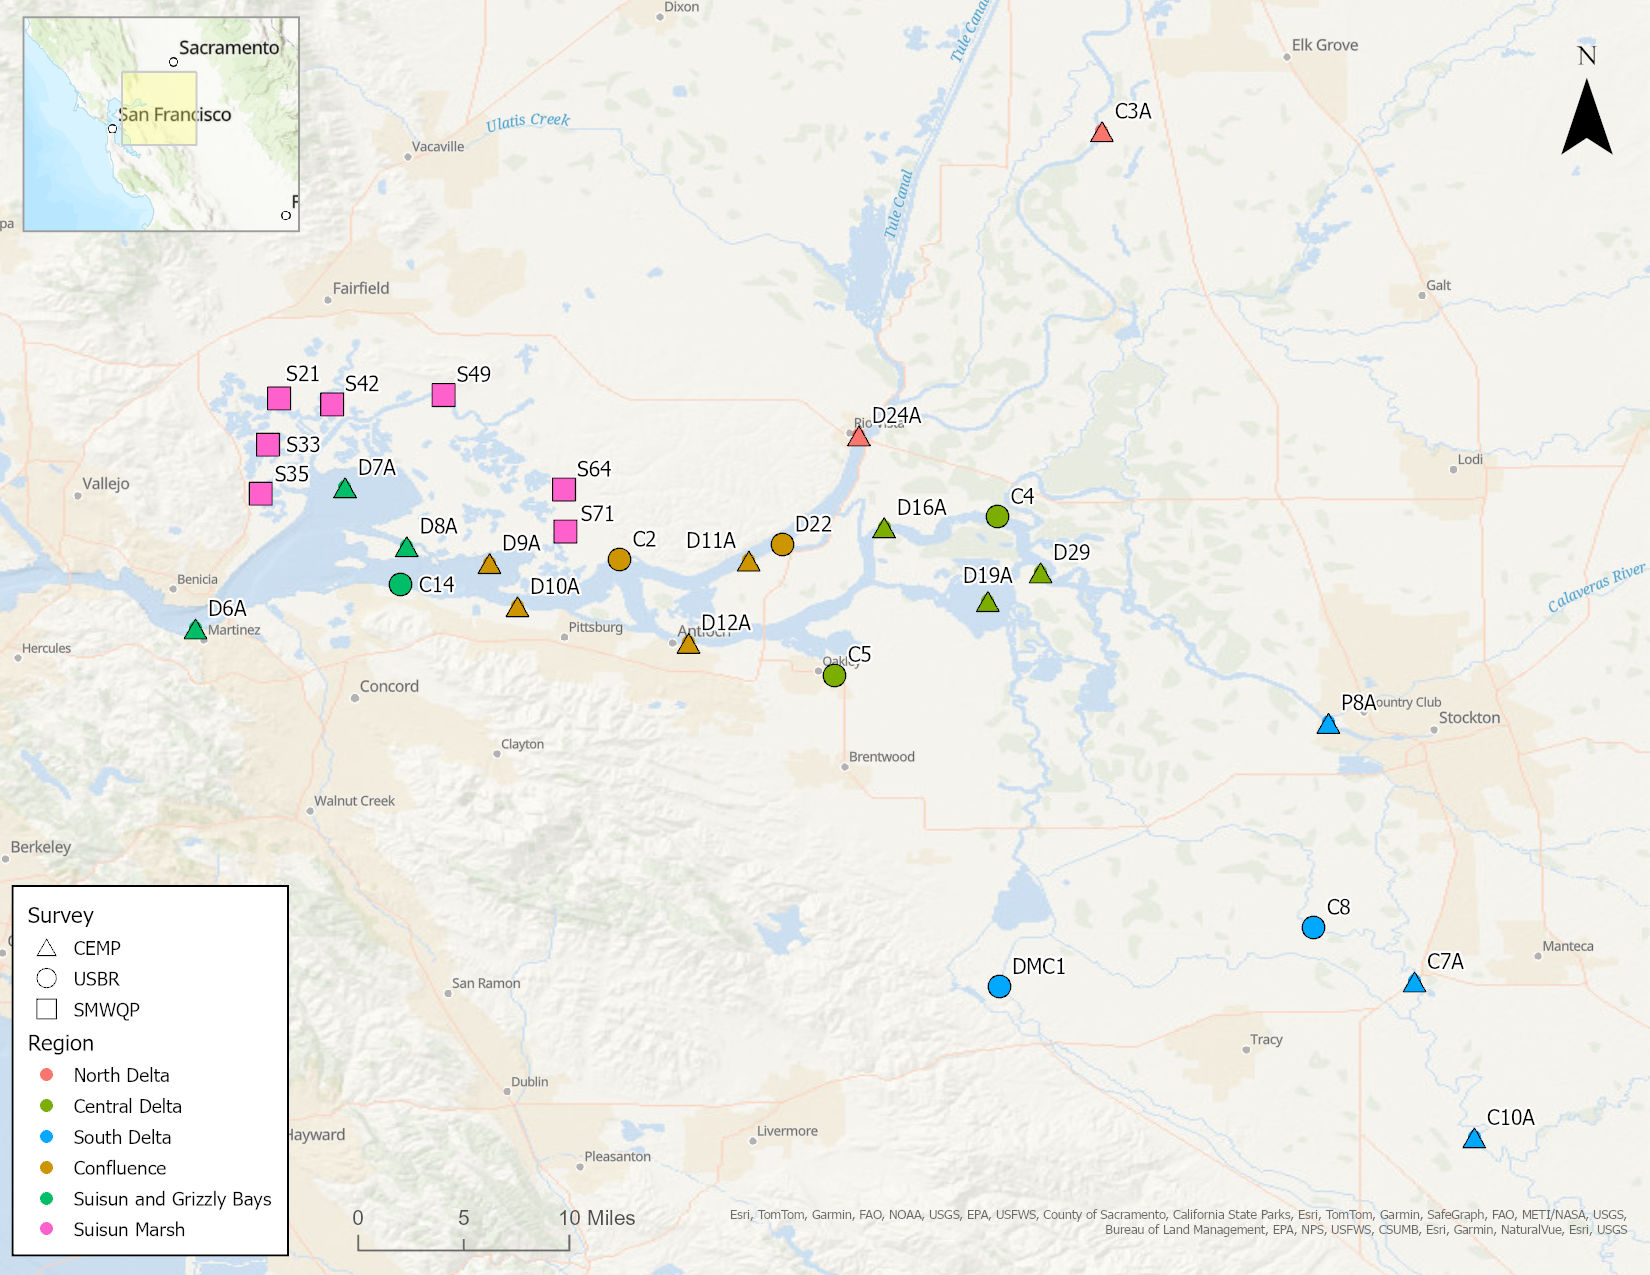
\includegraphics[width=1\linewidth,height=\textheight,keepaspectratio]{admin/figures-tables/cwq/cwq_station_map_pdf.jpg}

}

\caption{\label{fig-stations}Map of EMP's continuous WQ field sites}

\end{figure}%

\begin{figure}[H]

\centering{

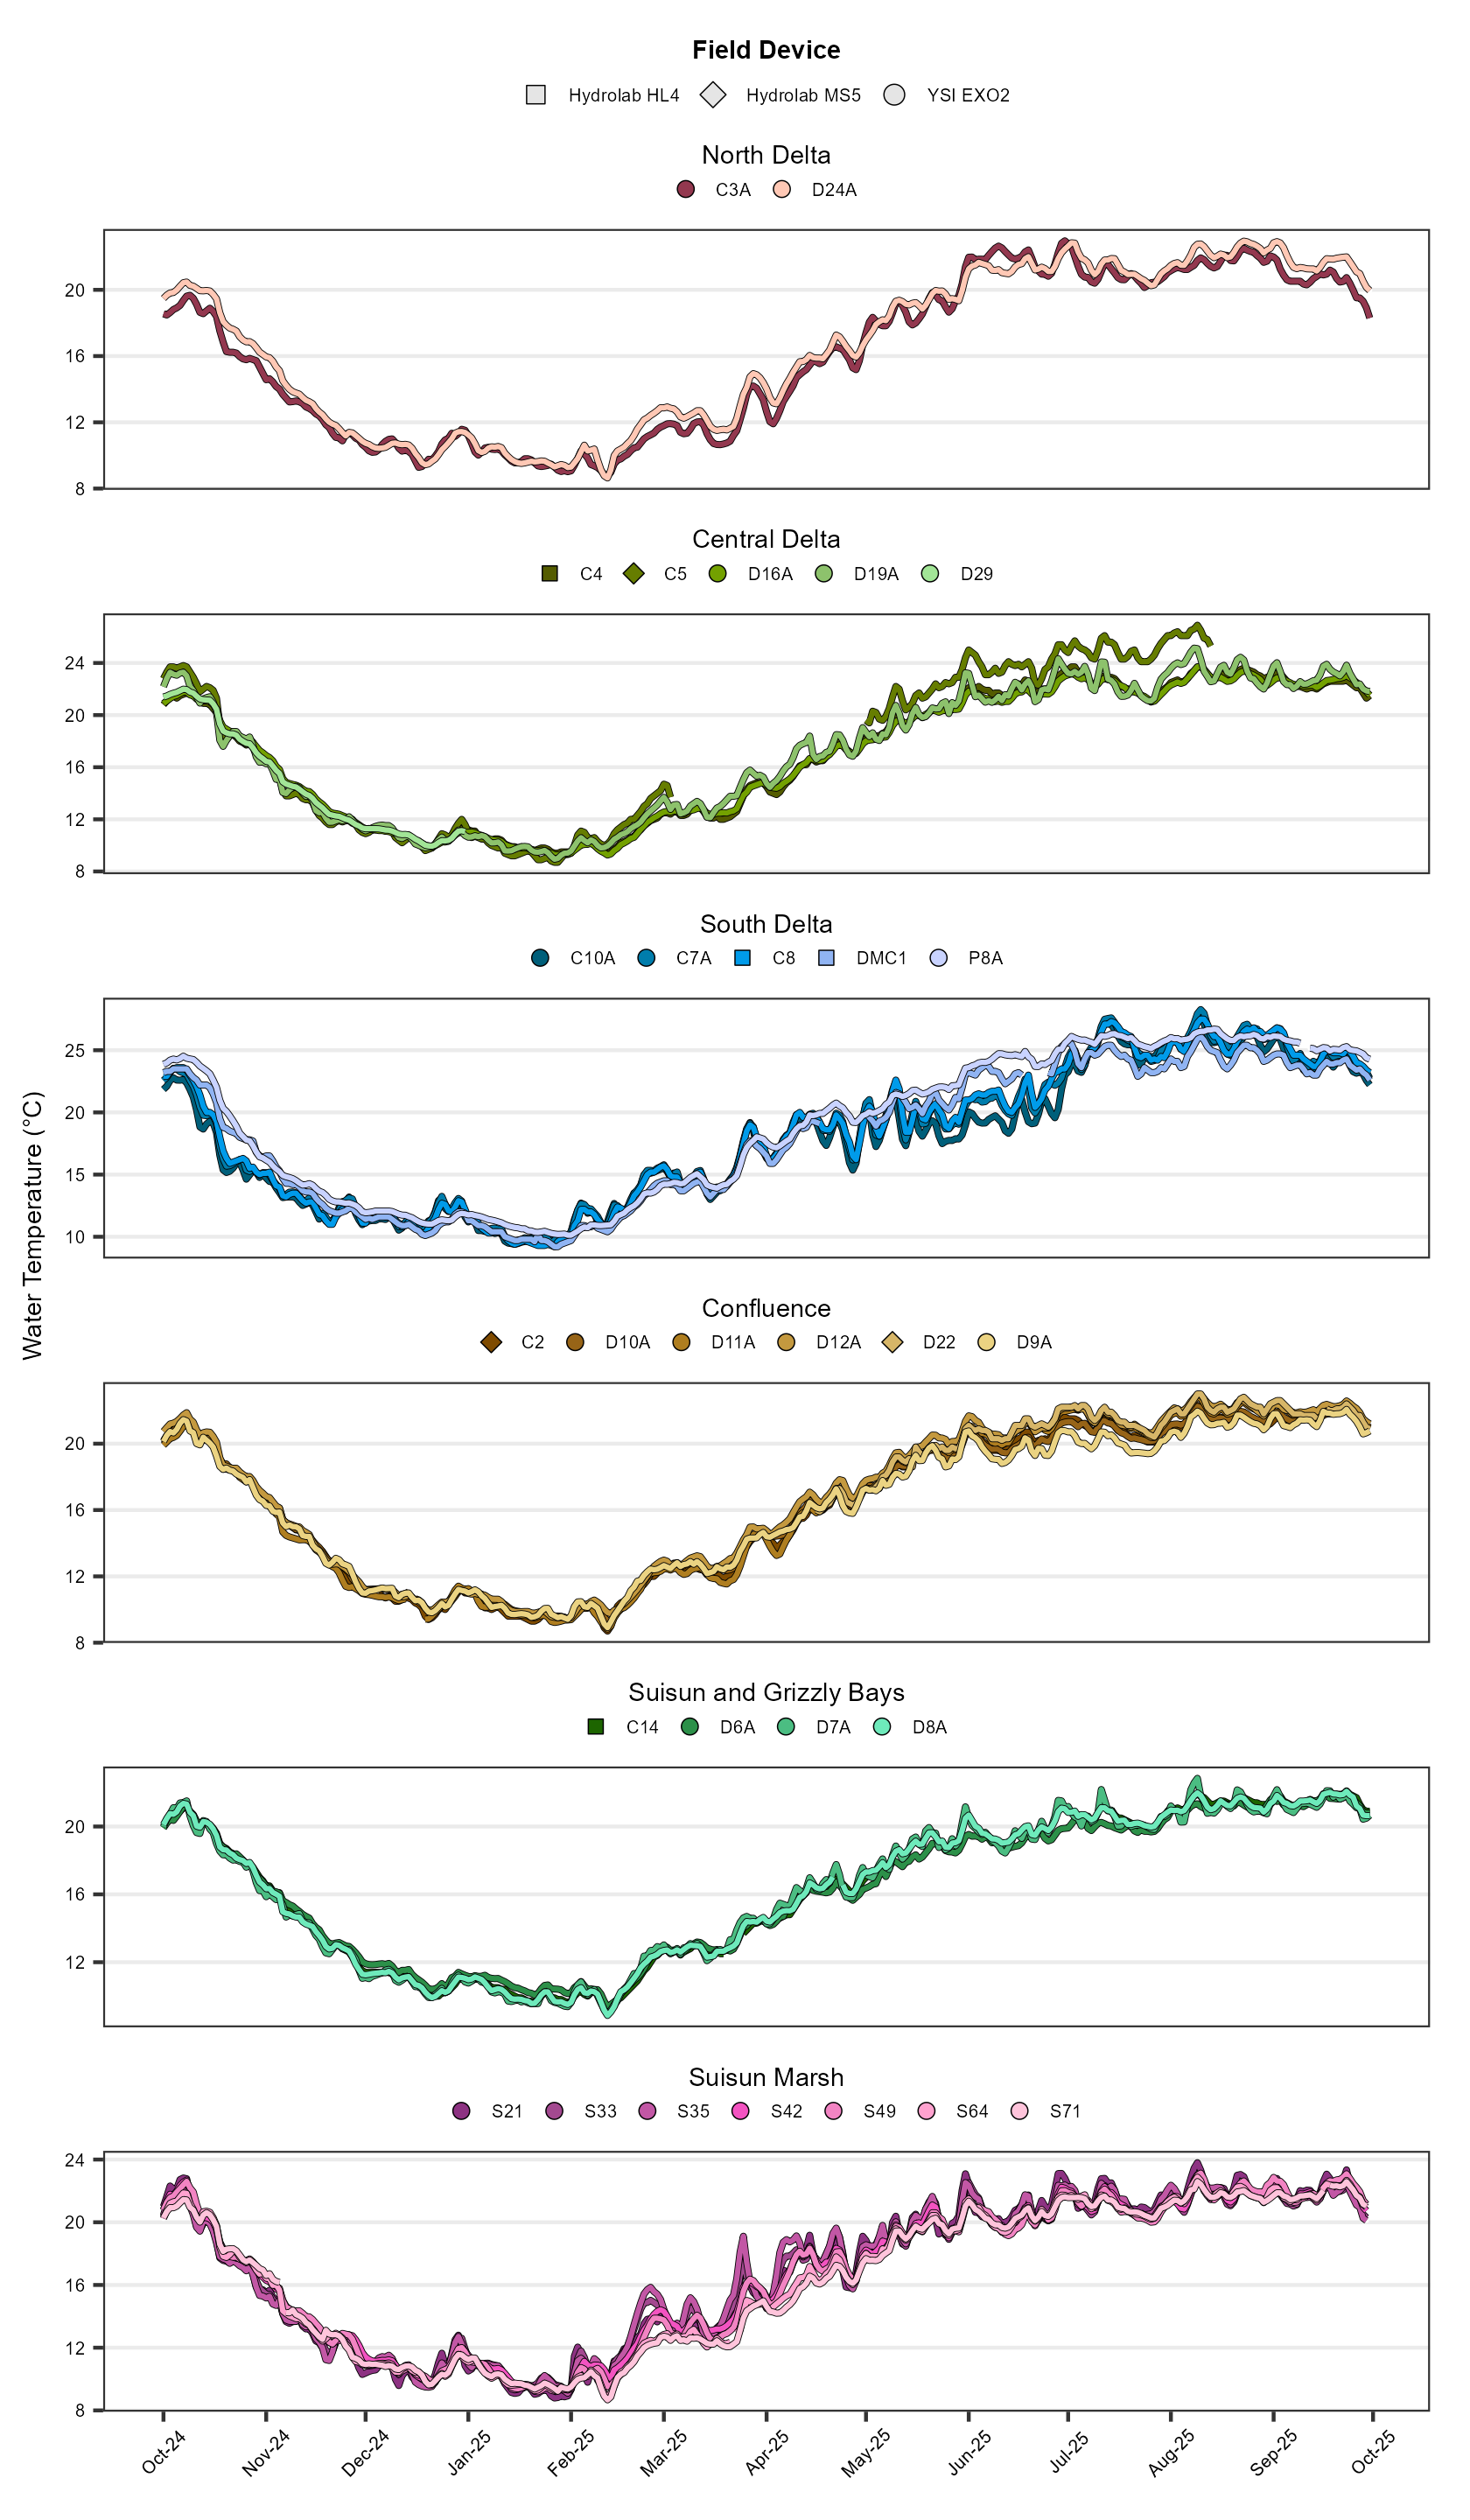
\includegraphics[width=5.6in,height=\textheight,keepaspectratio]{admin/figures-tables/cwq/cwq_ts_watertemperature.png}

}

\caption{\label{fig-watertemperature}Water temperature by region in the
San Francisco Bay-Delta estuary.}

\end{figure}%

\begin{figure}[H]

\centering{

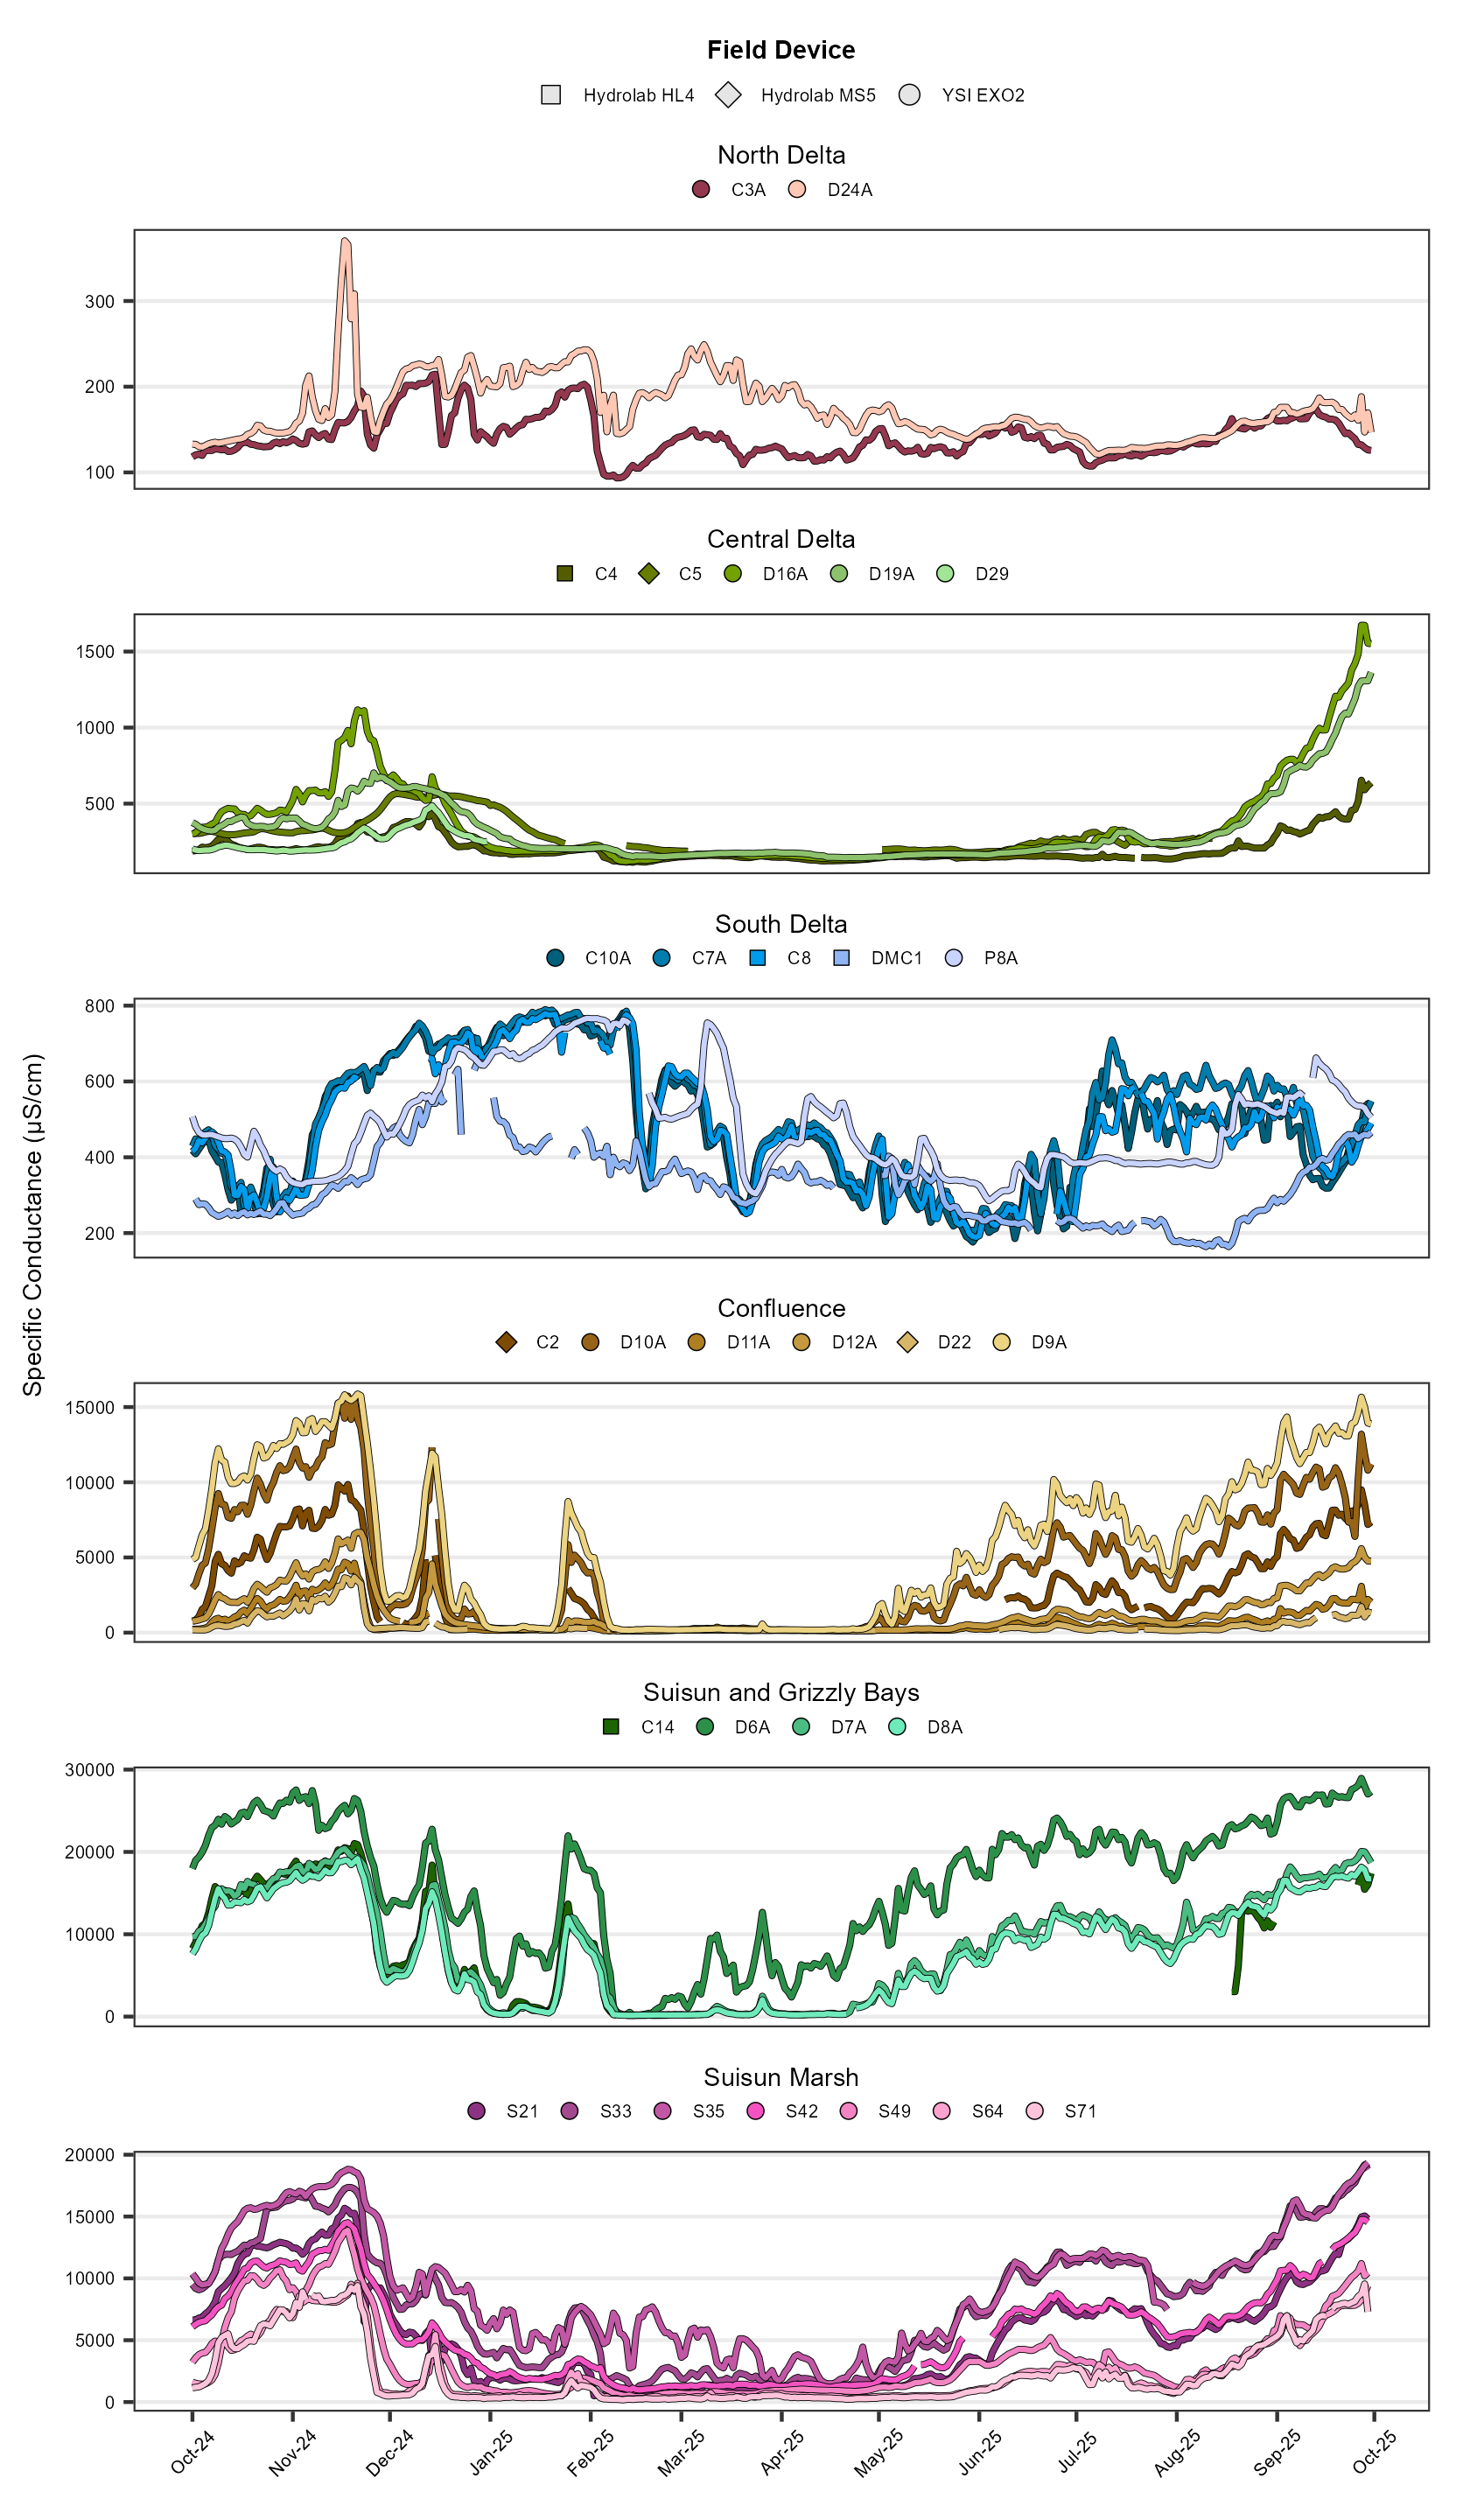
\includegraphics[width=5.6in,height=\textheight,keepaspectratio]{admin/figures-tables/cwq/cwq_ts_spc.png}

}

\caption{\label{fig-spc}Specific conductance by region in the San
Francisco Bay-Delta estuary.}

\end{figure}%

\begin{figure}[H]

\centering{

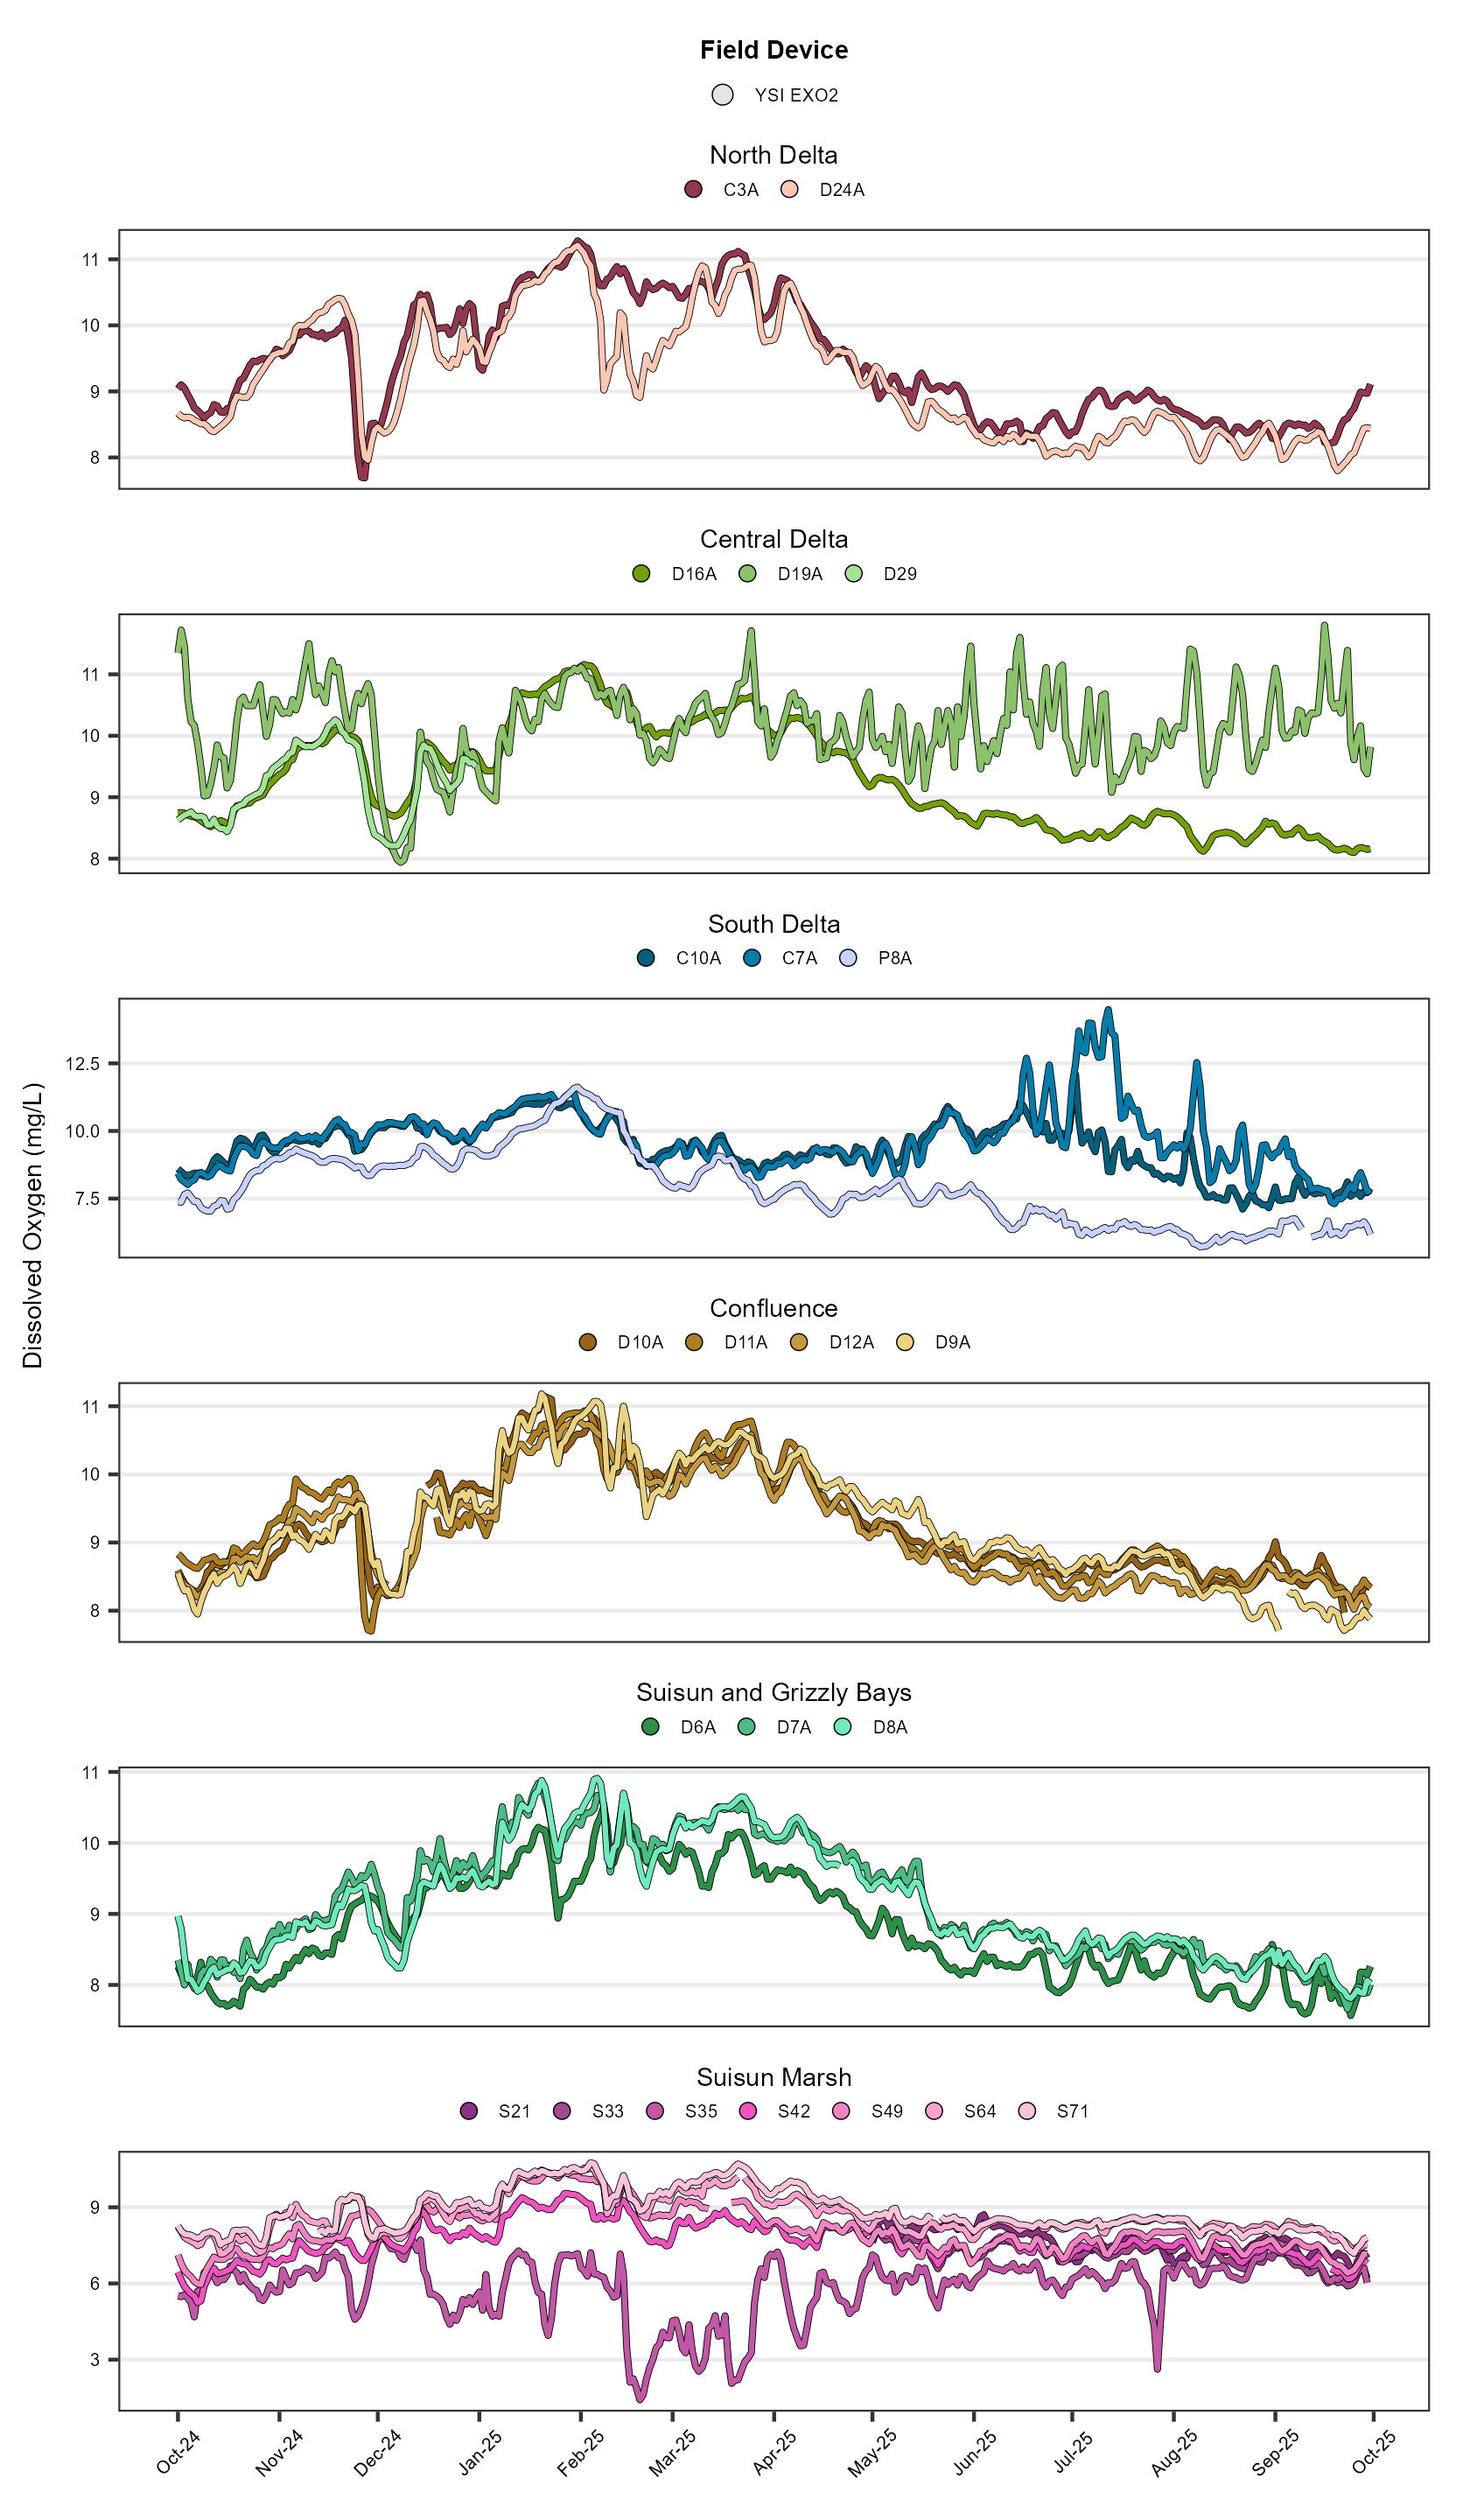
\includegraphics[width=5.6in,height=\textheight,keepaspectratio]{admin/figures-tables/cwq/cwq_ts_dissolvedoxygen.png}

}

\caption{\label{fig-dissolvedoxygen}Dissolved oxygen by region in the
San Francisco Bay-Delta estuary.}

\end{figure}%

\begin{figure}[H]

\centering{

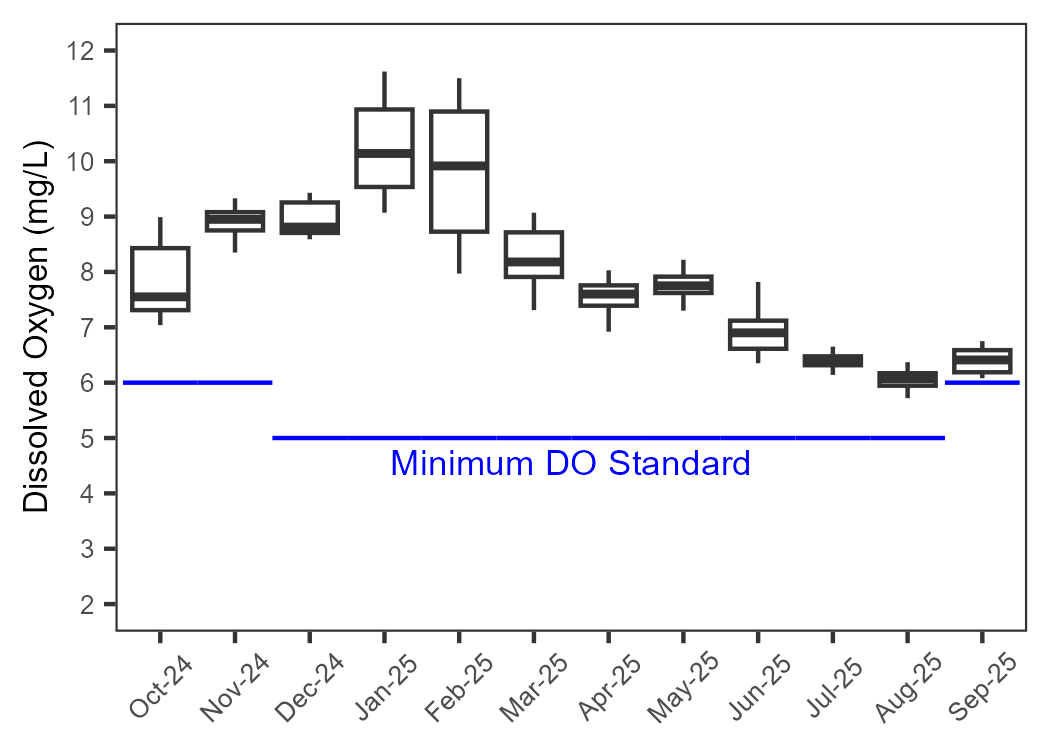
\includegraphics[width=3.5in,height=\textheight,keepaspectratio]{admin/figures-tables/cwq/cwq_rri_do.png}

}

\caption{\label{fig-rri}Range of daily dissolved oxygen values at the
Stockton Ship Channel (P8).}

\end{figure}%

\begin{figure}[H]

\centering{

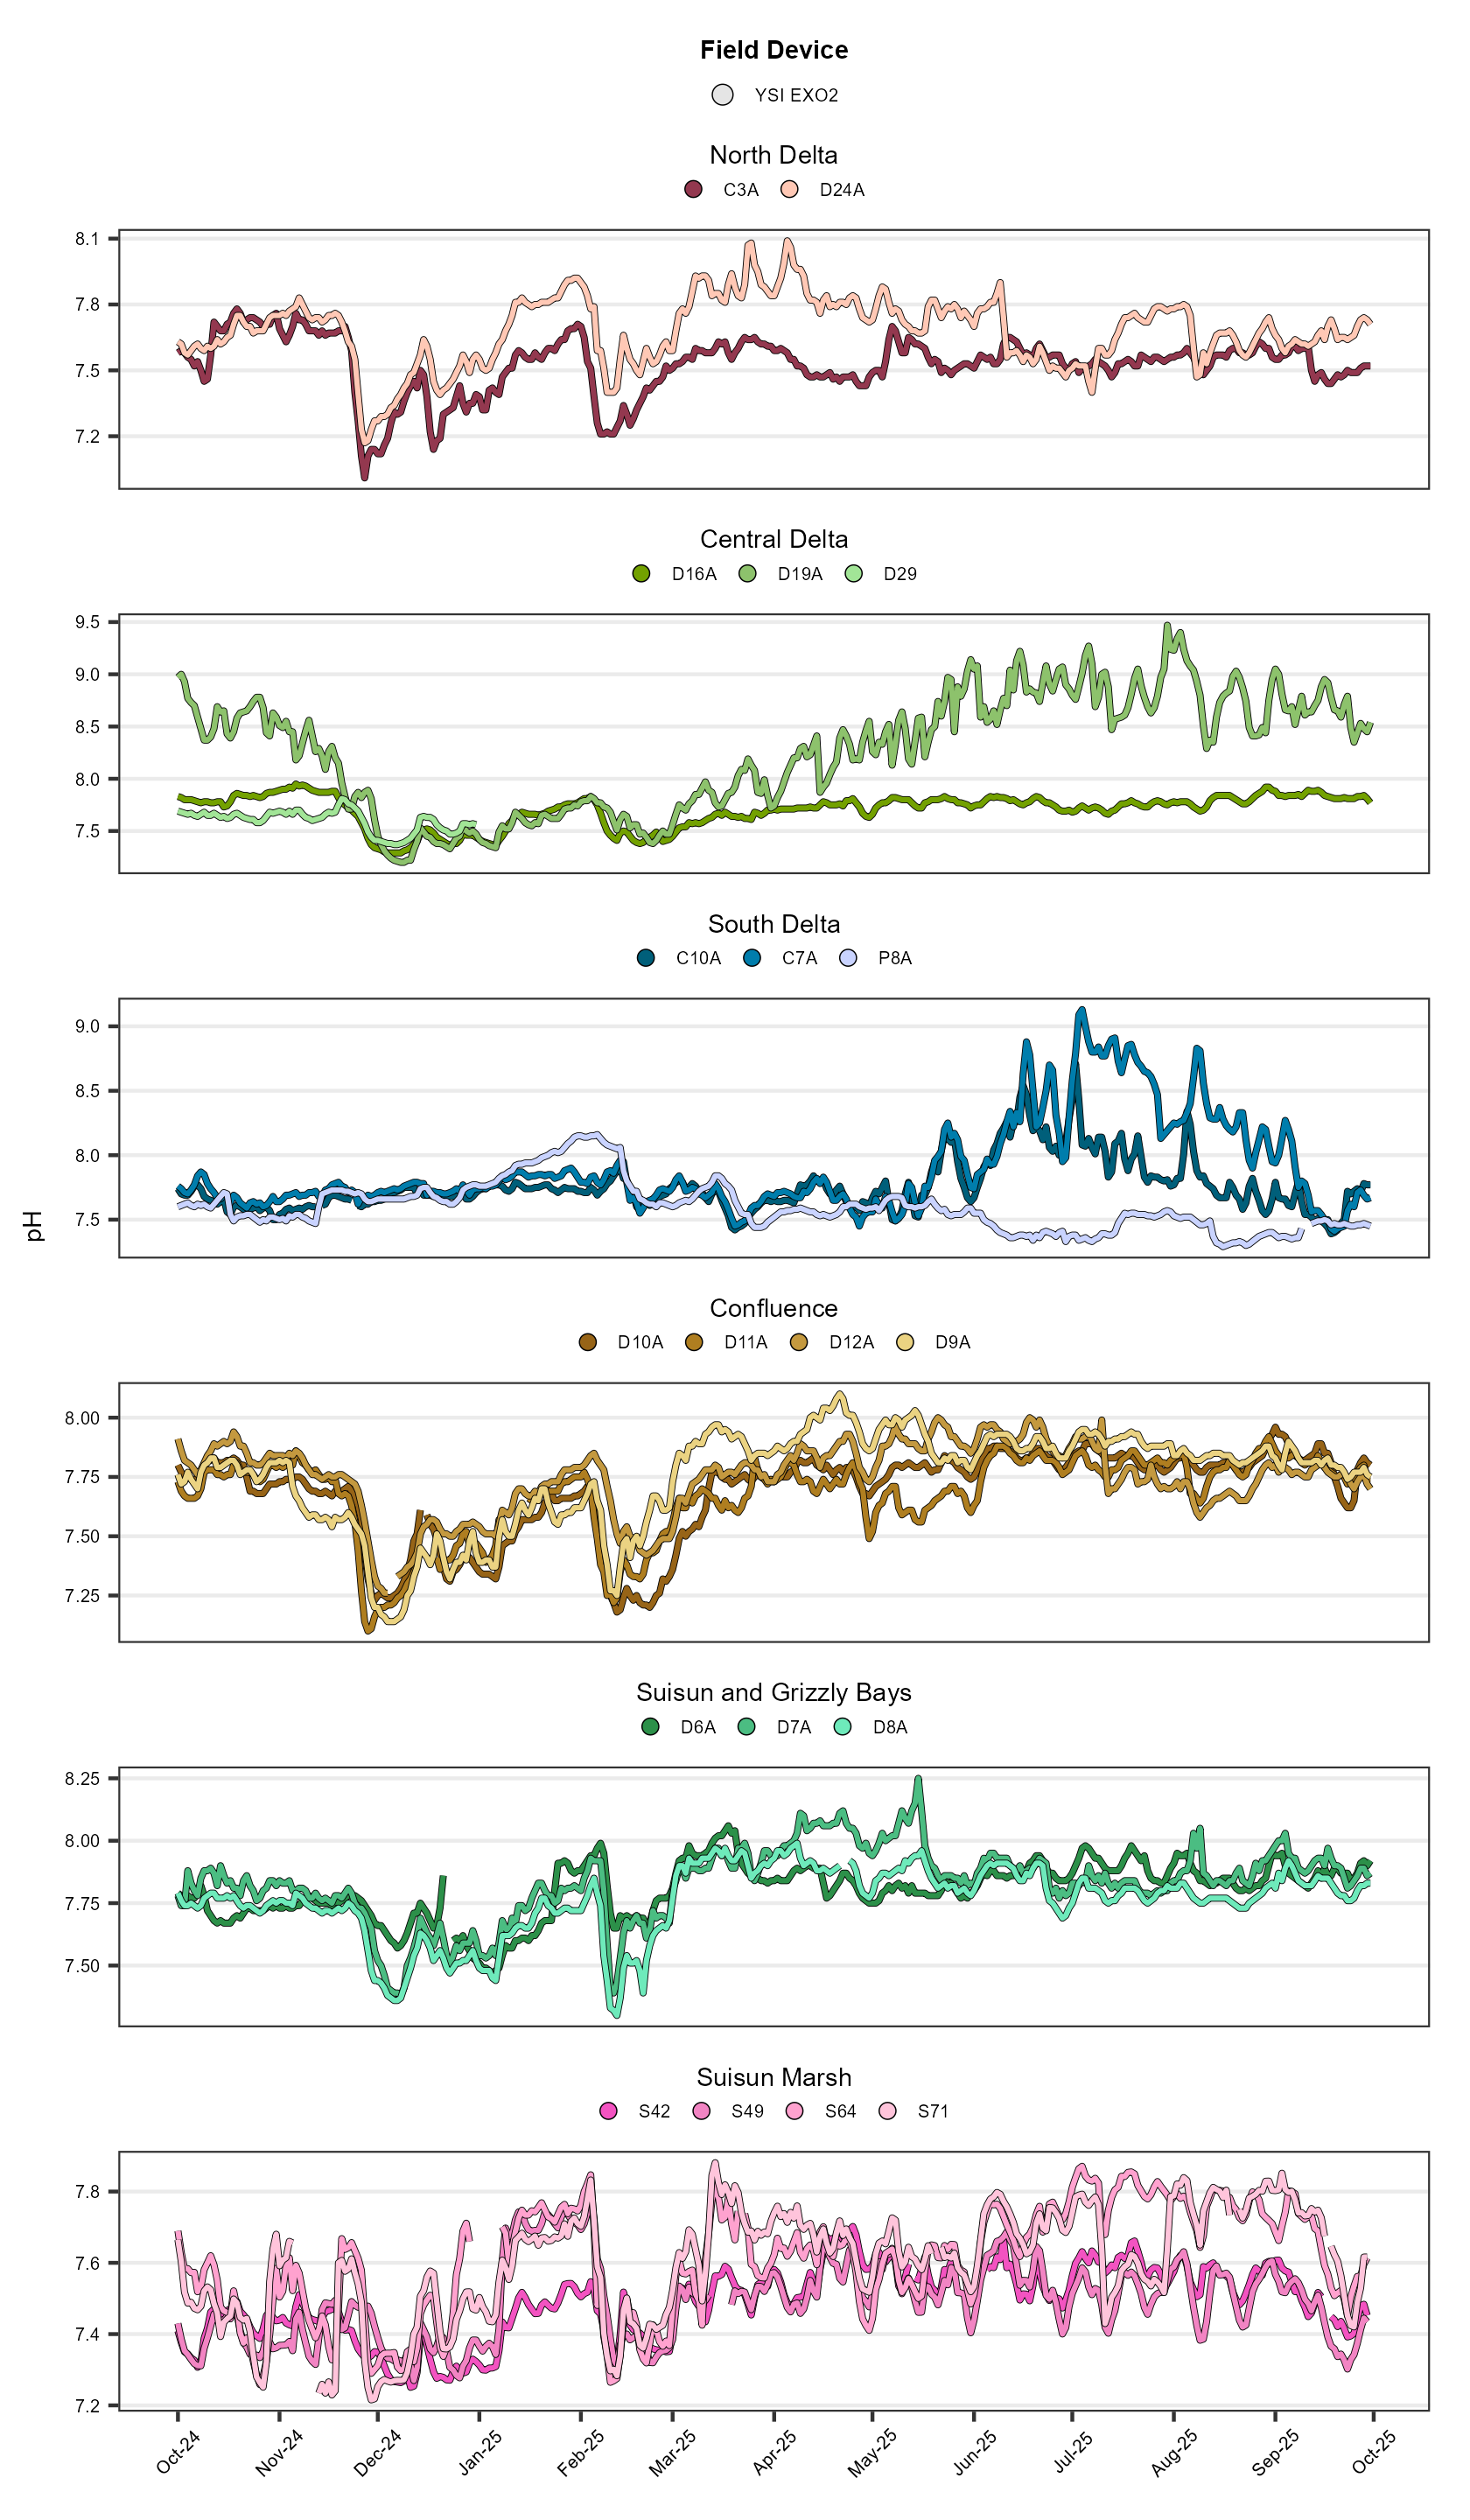
\includegraphics[width=5.6in,height=\textheight,keepaspectratio]{admin/figures-tables/cwq/cwq_ts_ph.png}

}

\caption{\label{fig-ph}pH by region in the San Francisco Bay-Delta
estuary.}

\end{figure}%

\begin{figure}[H]

\centering{

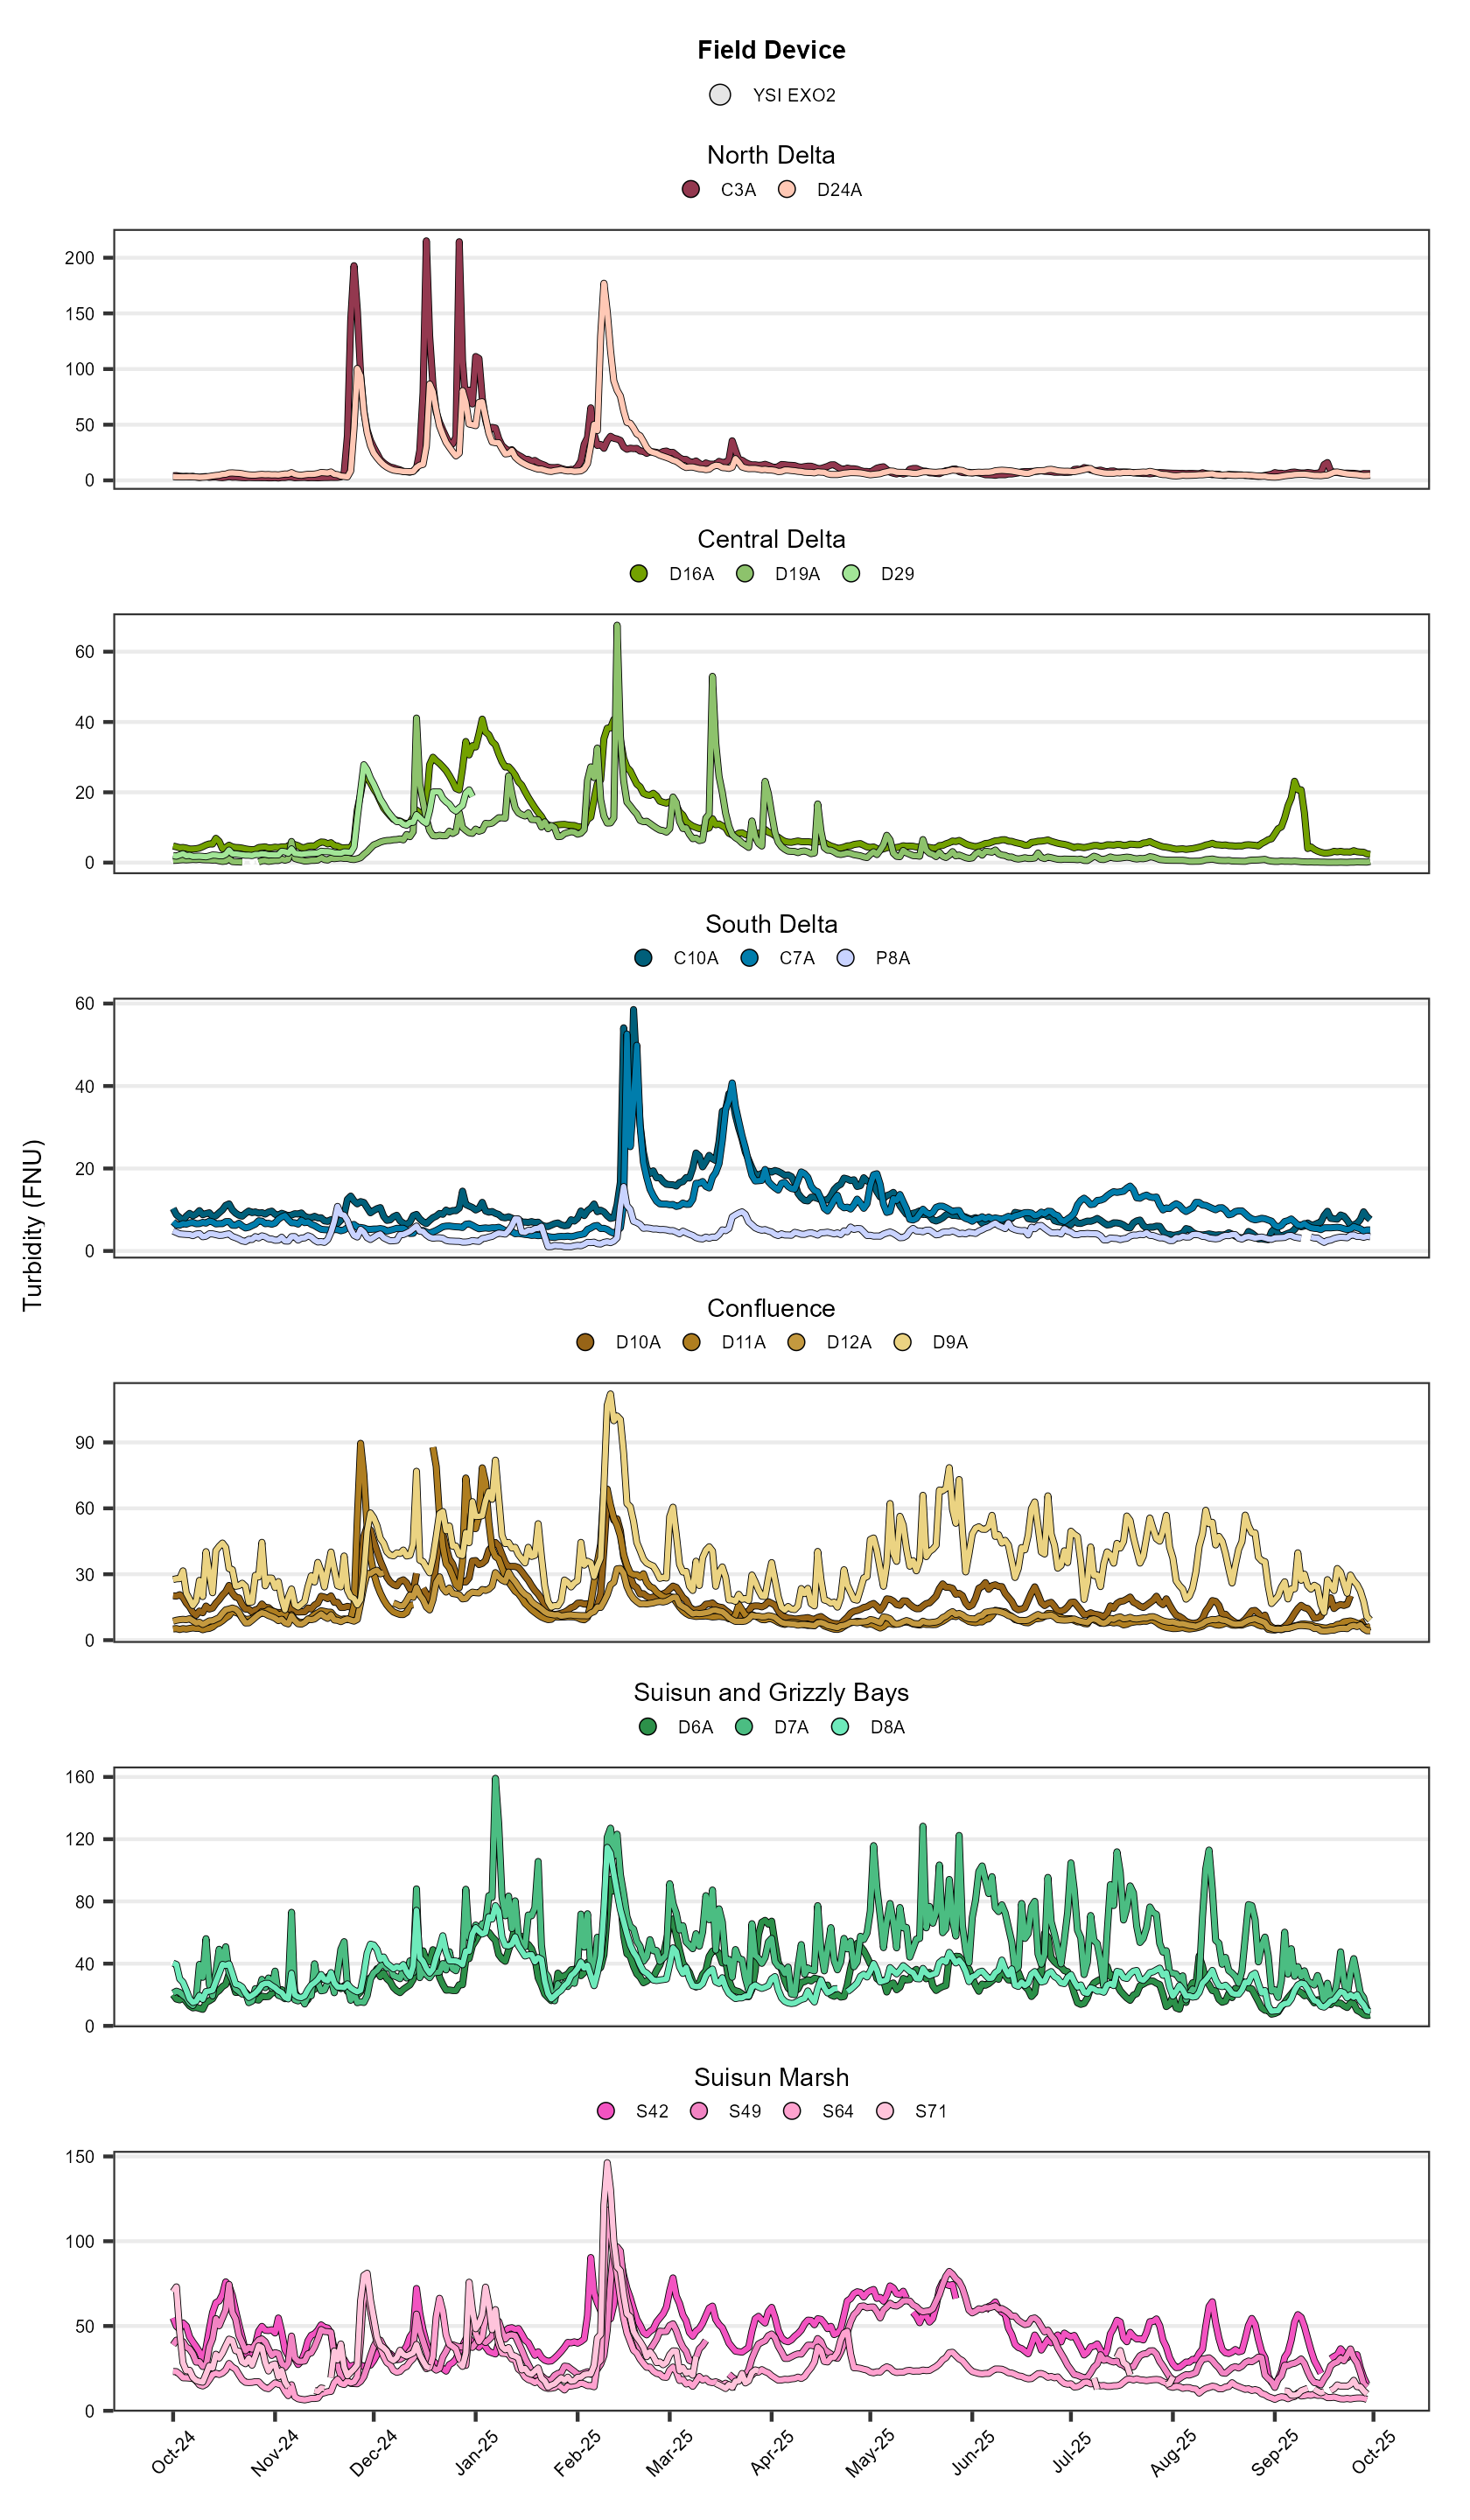
\includegraphics[width=5.6in,height=\textheight,keepaspectratio]{admin/figures-tables/cwq/cwq_ts_turbidity.png}

}

\caption{\label{fig-turbidity}Turbidity by region in the San Francisco
Bay-Delta estuary.}

\end{figure}%

\begin{figure}[H]

\centering{

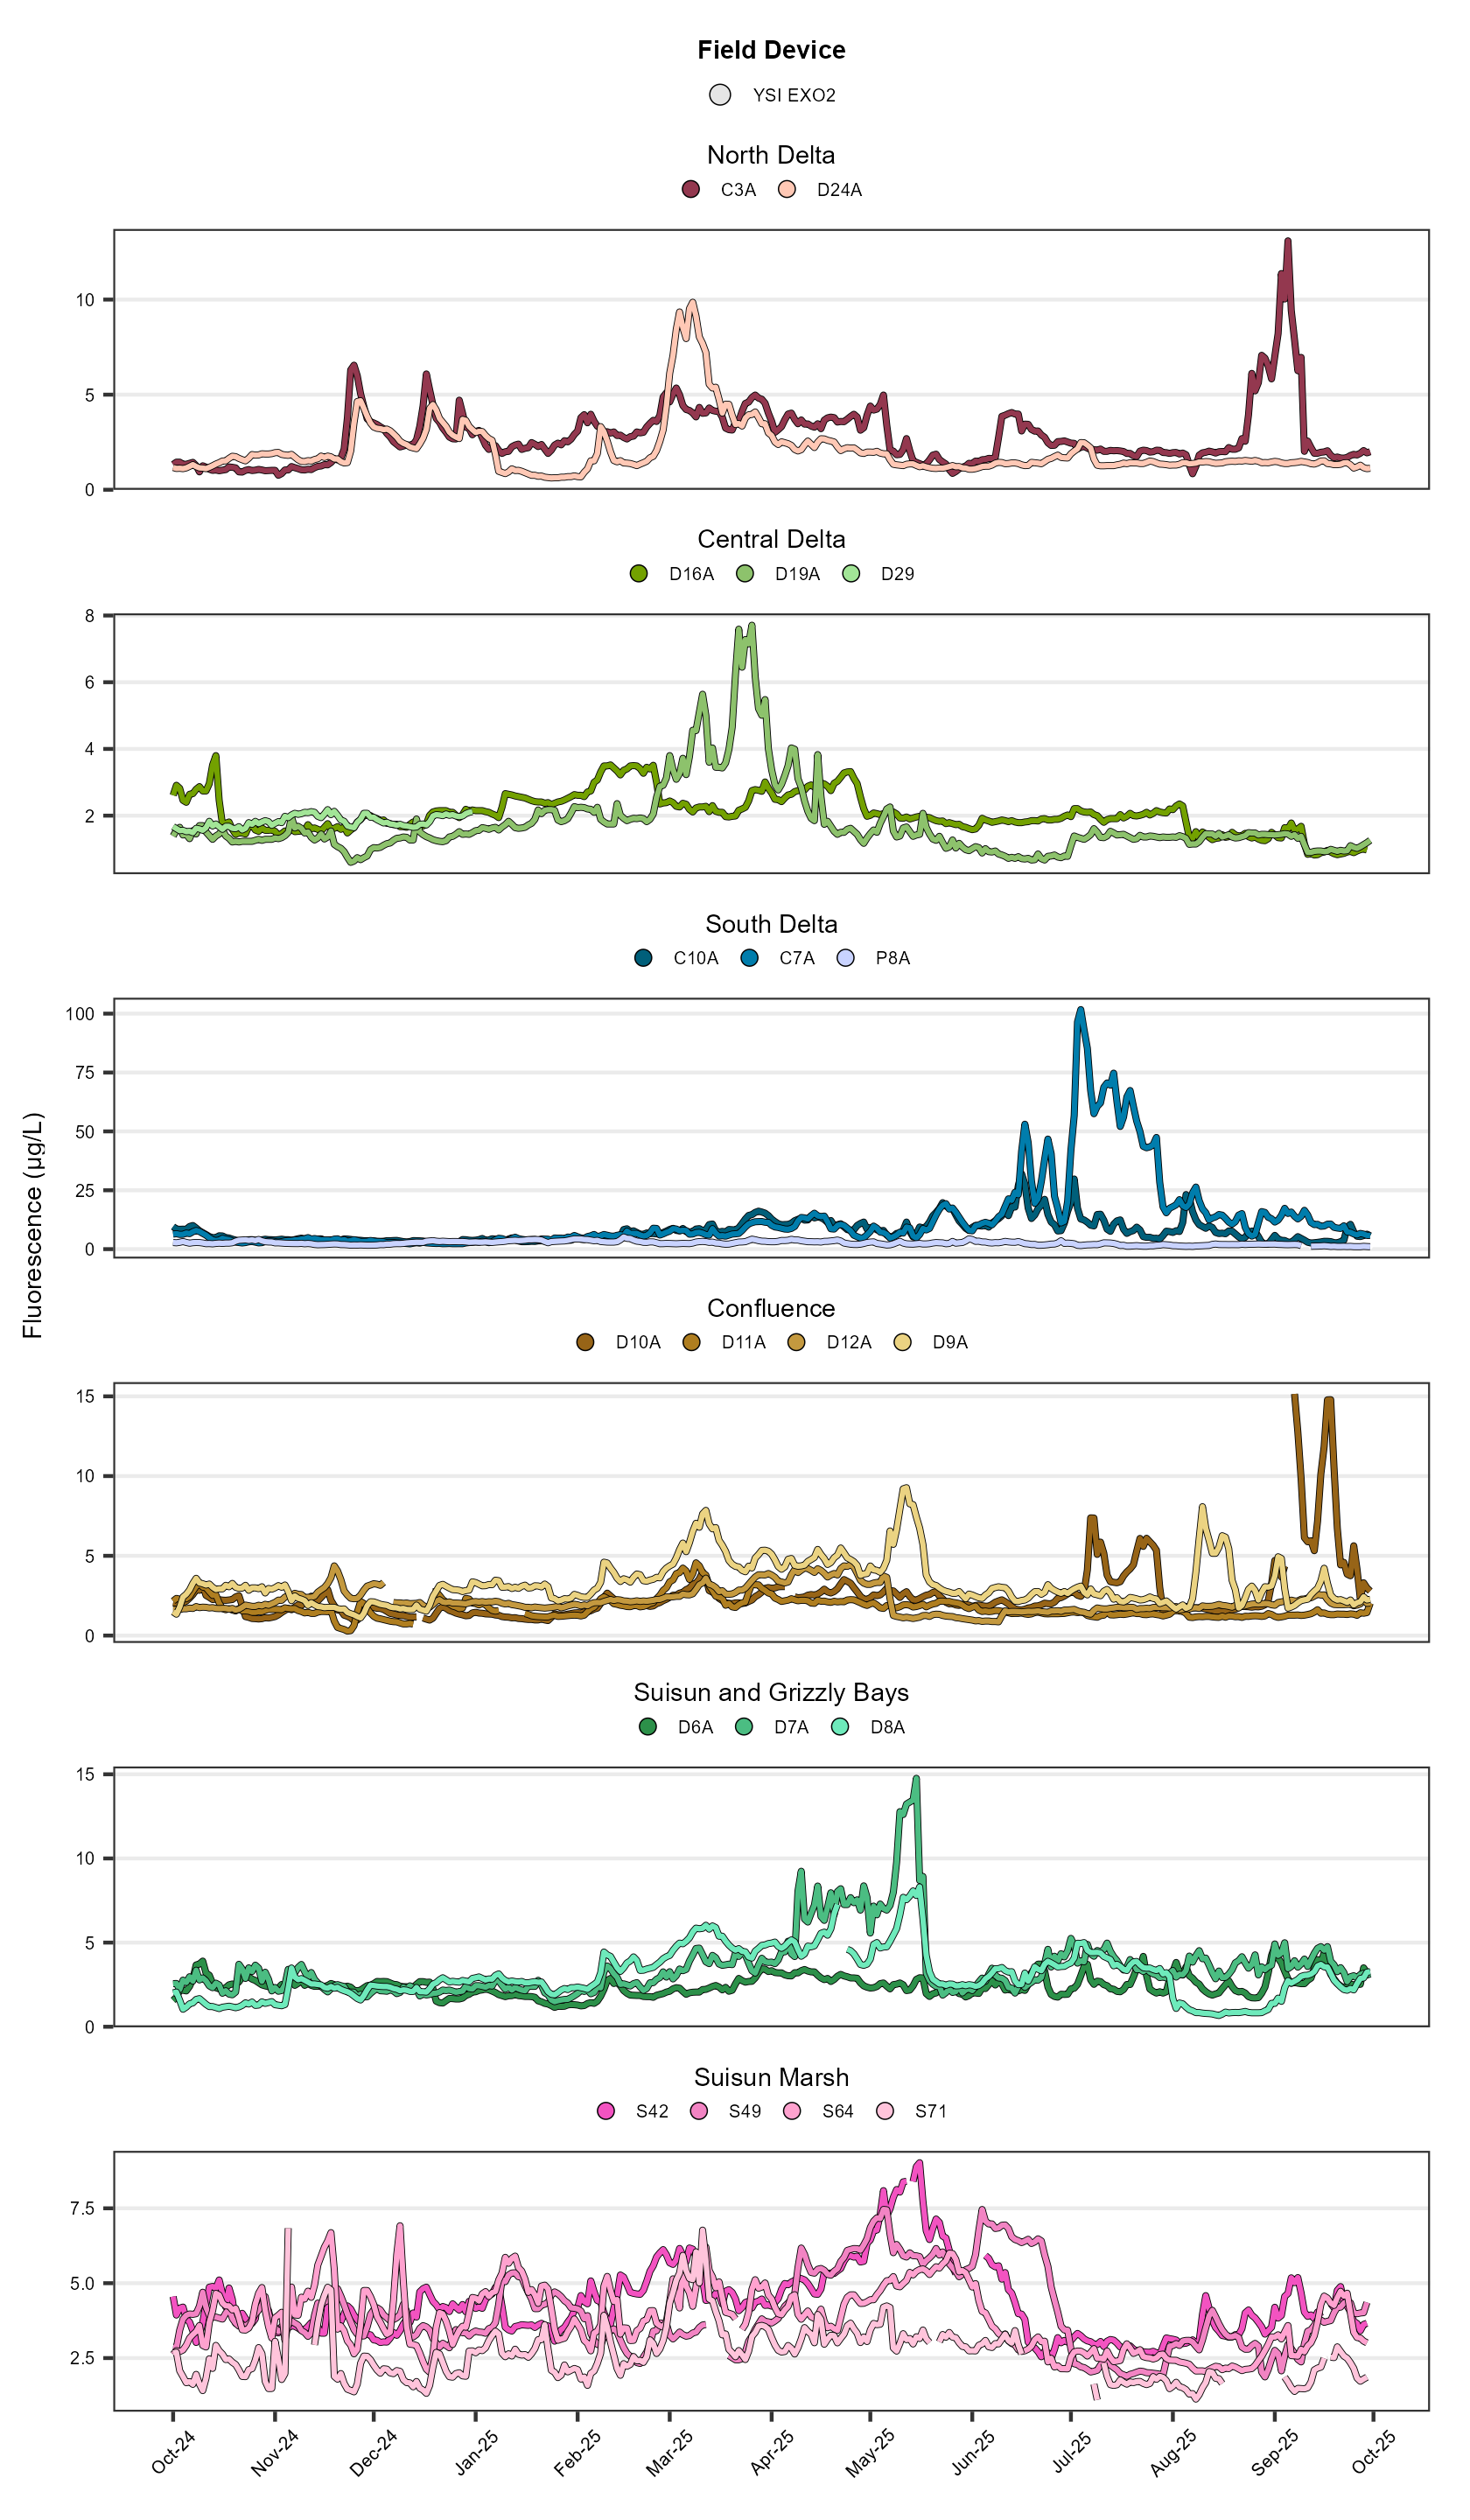
\includegraphics[width=5.6in,height=\textheight,keepaspectratio]{admin/figures-tables/cwq/cwq_ts_fluorescence.png}

}

\caption{\label{fig-fluorescence}Chlorophyll a fluorescence by region in
the San Francisco Bay-Delta estuary.}

\end{figure}%

\newpage

\section{Tables}\label{tables}

\begin{table}

\caption{\label{tbl-stations}Continuous WQ stations included within each
region of the Delta}

\centering{

\centering
\begin{tabular}{>{\centering\arraybackslash}p{11.6666666666667em}>{\centering\arraybackslash}p{11.6666666666667em}>{\centering\arraybackslash}p{11.6666666666667em}}
\toprule
Region & WY Index & Stations\\
\midrule
Central Delta & San Joaquin & C4, C5, D16A, D19A, D29\\
Confluence & Sacramento & C2, D9A, D11A, D12A, D22\\
North Delta & Sacramento & C3A, D24A\\
South Delta & San Joaquin & C7A, C8, C10A, DMC1, P8A\\
Suisun and Grizzly Bays & Sacramento & C14, D6A, D7A, D8A, D10A\\
\addlinespace
Suisun Marsh & Sacramento & S21, S33, S35, S42, S49, S64, S71\\
\bottomrule
\end{tabular}

}

\end{table}%

\begin{table}

\caption{\label{tbl-programs}List of device types used at continuous WQ
stations per program}

\centering{

\centering
\begin{tabular}{>{\centering\arraybackslash}p{17.5em}>{\centering\arraybackslash}p{17.5em}}
\toprule
Program & Stations\\
\midrule
DWR-EMP & C2, C3A, C7A, C10A, D6A, D7A, D8A, D9A, 
D10A, D11A, D12A, D16A, D19A, D24A, D29, P8A\\
DWR-SMWQP & S21, S33, S35, S42, S49, S64, S71\\
USBR-DWQMP & C2, C4, C5, C8, C14, D22, DMC1\\
\bottomrule
\end{tabular}

}

\end{table}%

\begin{table}

\caption{\label{tbl-watertemperature}Summary statistics for water
temperature by region in the San Francisco Bay-Delta estuary.}

\centering{

\centering
\begin{tabular}{>{\centering\arraybackslash}p{5em}>{\centering\arraybackslash}p{5em}>{\centering\arraybackslash}p{5em}>{\centering\arraybackslash}p{5em}>{\centering\arraybackslash}p{5em}>{\centering\arraybackslash}p{5em}>{\centering\arraybackslash}p{5em}}
\toprule
Statistic & Central Delta & Confluence & North Delta & South Delta & Suisun and Grizzly Bays & Suisun Marsh\\
\midrule
Average & 17.00 & 16.90 & 16.20 & 18.20 & 16.20 & 16.70\\
Min & 8.70 & 8.70 & 8.64 & 9.20 & 8.86 & 8.67\\
Max & 26.90 & 23.00 & 23.00 & 28.30 & 22.80 & 23.80\\
\bottomrule
\end{tabular}

}

\end{table}%

\begin{table}

\caption{\label{tbl-spc}Summary statistics for specific conductance by
region in the San Francisco Bay-Delta estuary.}

\centering{

\centering
\begin{tabular}{>{\centering\arraybackslash}p{5em}>{\centering\arraybackslash}p{5em}>{\centering\arraybackslash}p{5em}>{\centering\arraybackslash}p{5em}>{\centering\arraybackslash}p{5em}>{\centering\arraybackslash}p{5em}>{\centering\arraybackslash}p{5em}}
\toprule
Statistic & Central Delta & Confluence & North Delta & South Delta & Suisun and Grizzly Bays & Suisun Marsh\\
\midrule
Average & 300 & 2750 & 158 & 455 & 10700 & 5240\\
Min & 114 & 104 & 94 & 164 & 135 & 176\\
Max & 1670 & 15900 & 370 & 790 & 28900 & 19400\\
\bottomrule
\end{tabular}

}

\end{table}%

\begin{table}

\caption{\label{tbl-dissolvedoxygen}Summary statistics for dissolved
oxygen by region in the San Francisco Bay-Delta estuary.}

\centering{

\centering
\begin{tabular}{>{\centering\arraybackslash}p{5em}>{\centering\arraybackslash}p{5em}>{\centering\arraybackslash}p{5em}>{\centering\arraybackslash}p{5em}>{\centering\arraybackslash}p{5em}>{\centering\arraybackslash}p{5em}>{\centering\arraybackslash}p{5em}}
\toprule
Statistic & Central Delta & Confluence & North Delta & South Delta & Suisun and Grizzly Bays & Suisun Marsh\\
\midrule
Average & 9.66 & 9.23 & 9.32 & 9.00 & 9.04 & 7.75\\
Min & 7.94 & 7.70 & 7.69 & 5.72 & 7.57 & 1.42\\
Max & 11.80 & 11.20 & 11.30 & 14.50 & 10.90 & 10.80\\
\bottomrule
\end{tabular}

}

\end{table}%

\begin{table}

\caption{\label{tbl-ph}Summary statistics for pH by region in the San
Francisco Bay-Delta estuary.}

\centering{

\centering
\begin{tabular}{>{\centering\arraybackslash}p{5em}>{\centering\arraybackslash}p{5em}>{\centering\arraybackslash}p{5em}>{\centering\arraybackslash}p{5em}>{\centering\arraybackslash}p{5em}>{\centering\arraybackslash}p{5em}>{\centering\arraybackslash}p{5em}}
\toprule
Statistic & Central Delta & Confluence & North Delta & South Delta & Suisun and Grizzly Bays & Suisun Marsh\\
\midrule
Average & 7.94 & 7.71 & 7.60 & 7.75 & 7.80 & 7.55\\
Min & 7.20 & 7.10 & 7.01 & 7.29 & 7.30 & 7.22\\
Max & 9.47 & 8.10 & 8.09 & 9.13 & 8.25 & 7.88\\
\bottomrule
\end{tabular}

}

\end{table}%

\begin{table}

\caption{\label{tbl-turbidity}Summary statistics for turbidity by region
in the San Francisco Bay-Delta estuary.}

\centering{

\centering
\begin{tabular}{>{\centering\arraybackslash}p{5em}>{\centering\arraybackslash}p{5em}>{\centering\arraybackslash}p{5em}>{\centering\arraybackslash}p{5em}>{\centering\arraybackslash}p{5em}>{\centering\arraybackslash}p{5em}>{\centering\arraybackslash}p{5em}}
\toprule
Statistic & Central Delta & Confluence & North Delta & South Delta & Suisun and Grizzly Bays & Suisun Marsh\\
\midrule
Average & 7.70 & 20.40 & 15.90 & 8.16 & 37.30 & 34.60\\
Min & 0.08 & 4.12 & 2.17 & 1.03 & 6.69 & 6.46\\
Max & 67.50 & 112.00 & 215.00 & 58.50 & 159.00 & 146.00\\
\bottomrule
\end{tabular}

}

\end{table}%

\begin{table}

\caption{\label{tbl-fluorescence}Summary statistics for chlorophyll a
fluorescence by region in the San Francisco Bay-Delta estuary.}

\centering{

\centering
\begin{tabular}{>{\centering\arraybackslash}p{5em}>{\centering\arraybackslash}p{5em}>{\centering\arraybackslash}p{5em}>{\centering\arraybackslash}p{5em}>{\centering\arraybackslash}p{5em}>{\centering\arraybackslash}p{5em}>{\centering\arraybackslash}p{5em}}
\toprule
Statistic & Central Delta & Confluence & North Delta & South Delta & Suisun and Grizzly Bays & Suisun Marsh\\
\midrule
Average & 1.90 & 2.45 & 2.46 & 7.75 & 3.04 & 3.72\\
Min & 0.60 & 0.28 & 0.62 & 1.03 & 0.67 & 1.11\\
Max & 7.71 & 15.20 & 13.10 & 102.00 & 14.80 & 9.02\\
\bottomrule
\end{tabular}

}

\end{table}%




\end{document}
